\documentclass[11pt]{article}

\usepackage{amssymb}
\usepackage[english]{babel}
\usepackage{changepage}
\usepackage{cite}
\usepackage{float}
\usepackage[margin=1.5in]{geometry}
\usepackage{graphicx}
\usepackage{lmodern}
\usepackage{setspace}
\usepackage{tabularx}
\usepackage[table,xcdraw]{xcolor}
\usepackage{adjustbox}
\usepackage{url}

\usepackage{indentfirst}

\usepackage[T1]{fontenc}

\bibliographystyle{ieeetr}

\graphicspath{{figures}}

\onehalfspacing

\begin{document}
\thispagestyle{empty}
\begin{center}
\begin{Large}
\emph{Master's of Science Thesis Proposal} \\
Department of Computer Science \\
Rochester Institute of Technology \\
\end{Large}
\vspace{4em}
{\huge Generalized Model of Cognitive Workload} \\
\vspace{3em}
{\LARGE Taylor Carpenter} \\
{\tt tjc1575@rit.edu} \\
\vspace{3em}
\begin{adjustwidth}{.5in}{.5in}
Chair: Dr. Zack Butler \hfill {\tt zjb@cs.rit.edu} \\
\vspace{2em}
\hrulefill \\
\vspace{3em}
Reader: Dr. Esa Rantanen \hfill {\tt emrgsh@rit.edu} \\
\vspace{2em}
\hrulefill \\
\vspace{3em}
Observer: Sean Strout \hfill {\tt sps@cs.rit.edu} \\
\vspace{2em}
\hrulefill
\end{adjustwidth}
\vspace{2em}
Rochester, NY 14623 USA \\
\vspace{2em}
\today
\end{center}
\pagebreak
\thispagestyle{empty}
\begin{abstract}
\noindent
Human operators are commonly involved in complex human-machine systems that are present in many industries. The topic of cognitive workload monitoring of system operators has been a popular focal point of many studies over the past few decades. The ability to determine the load of an individual performing a task would allow for a more in-depth analysis of how the task affects the operator and also more sophisticated adaptive automation. While cognitive workload estimators have been well explored, they are commonly individualized models that are restricted to a single task. Unfortunately, these models are of little use outside of a controlled lab setting as they require too much time to train and are too specific. In this thesis, we will explore the practicality of a generalized cognitive workload model. Using psychophysiological data collected from individuals as they perform two cognitive loading tasks at varying difficulty levels, a model will be trained independent of individual and task. The effectiveness of said model will be compared to existing, non-generalized models of cognitive workload. 
\end{abstract}
\clearpage
\pagenumbering{arabic}
\tableofcontents
\listoffigures
\listoftables
\pagebreak

\section{Introduction}
Human operators are commonly involved in complex human-machine systems that are present in many industries. Researchers from many fields have advanced the abilities of automation to the point where it is found in a variety of fields. Similar to computers, humans have a limited amount of resources that can be dedicated towards a specific task. When the resources are under heavy load, or in the case of a person, when they are overworked mentally, suboptimal decisions and errors can occur. This degradation in performance can lead to serious disasters~\cite{Wickens}. In many cases, it can be difficult to detect the degradation of the operator's effectiveness as primary task performance will be maintained while secondary tasks receive less attention~\cite{Hockey}.  Unlike a computer system, however, methods for monitoring the working state of human operators have not been well developed. The cognitive workload of a person is more difficult to quantify than stress on a computer. If a system can be developed to monitor the functional state of a person, load balancing methods can be used to transfer work to other human operators, or to autonomous systems through adaptive automation~\cite{Wilson}. Effective monitoring of cognitive workload could reduce overall system errors and remove unnecessary stress from operators. High workload is not the only condition that can lead to errors in a human-machine system. In cases of low workload, operators can become complacent and miss signals that must be addressed due to low vigilance~\cite{Parasuraman}. Thus, an effective cognitive workload monitor must be able to detect multiple levels of cognitive workload.

\subsection{Definitions}
Many definitions exist for cognitive workload as it is a theoretical concept that is intuitive to understand but difficult to fully encapsulate within a single statement. For the purposes of this research, the definition of cognitive workload is that proposed by Meshkati: ``mental workload [is] a multidimensional construct that reflects the interaction of such elements as task and system demands, operator processing capabilities and effort, subjective performance criteria, operator information processing behavior and strategies, and finally, operator training and prior experience.''~\cite{Meshkati}. Since mental workload is a theoretical construct that exists in the mind, there are no methods of measuring the load directly. Instead, loading tasks can be used to affect workload while measurements, such as various psychophysiological readings, can be examined that allow for inferences to be made about cognitive workload. With respect to this study, descriptions about measuring cognitive workload are in fact referring to the indirect measurement of factors affected by workload and making inferences about the underlying load. Another term commonly used in this line of research is ``operator functional state'' or OFS. The definition of OFS used in this study is that put forth by Hockey: ``the variable capacity of the operator for effective task performance in response to task and environmental demands, and under the constraints imposed by cognitive and physiological processes that control and energize behavior''~\cite{Hockey}. In many applications, such as this study and various other similar studies, cognitive workload and OFS can be seen as the same construct and used interchangeably. For the sake of clarity, cognitive workload is the term that will be used throughout this research. Another term that will be used throughout this research is ``model''. In this case, the more mathematical definition of model that is used in the context of machine learning is intended, rather than a strictly psychological definition. A model, as used in machine learning, is a system that can take in input data and produce some output as defined by patterns present in historical data. This system may be a black-box or it may be described with well defined rules, depending on the technique used.

\section{Related Work}
Classifying cognitive workload has been the subject of many studies. The majority of studies deal with creating an individual model unique to each participant in the study, with the study consisting of only one task. The use of EEG and heart rate as psychophysiological features is common for models in cognitive workload studies~\cite{Wang_R, Zhang, Wilson, Yang}. Features involving EEG can be generated in a variety of ways. Some of the studies, such as the work performed by Wilson et al.~\cite{Wilson}, use log power of spectral information from the EEG measurements while other studies, such as that by Zhang et al.~\cite{Zhang}, use combinations of EEG spectral information, called task load indices. In addition to EEG and heart rate, some studies include blink rate~\cite{Wilson, Wilson_2002} and respiration rate~\cite{Wilson_2003} as features. Other studies used blinking and eye movement measures to correct artifacts in EEG data~\cite{Wang_R}. The general layout for each of the studies was roughly the same; participants were attached to a variety of sensors and then asked to perform a loading task at varying difficulty levels to induce different cognitive workloads. The two most common loading tasks used were MATB~\cite{Estepp} and AutoCAMS~\cite{Lorenz}. These systems are commonly used due to their ability to systematically vary the difficulty settings. 

A variety of different classifiers have been used in studies in an attempt to model cognitive workload. The study covered by Yang et al.~\cite{Yang} uses a system of fuzzy inference rules to perform realtime classification of cognitive workload for the purposes of adaptive automation triggering. An SVM Regressor was used by Ke et al.~\cite{Ke} to produce a cognitive workload index, a particular number corresponding to cognitive workload level. Another study~\cite{Wang_R} explored the use of an Adaptive-Network-based Fuzzy Inference System that was trained using differential evolution and ant colony search as a means of predicting levels of cognitive workload. Fuzzy C-Means clustering was used in a study~\cite{Zhang} as a means of classification through clustering. The study completed by Wilson et al.~\cite{Wilson} used an artificial neural network. All of these studies have shown adequate results but have failed to address the larger scope of generalizability. One study~\cite{Wang_Z} used a bayesian model to explore the ability of a model to be used on multiple subjects, learning from and tested on a dataset consisting of data from multiple participants. What the study lacked, however, was the ability to handle novel data; that is, classify on a participant that was previously unseen. A different study~\cite{Ke} falls in a similar category, however it deals with multiple tasks rather than multiple participants. The study involved testing on data from an unseen task,  showing the possibility for full generalization. An additional study~\cite{Christensen} demonstrated how cognitive workload metrics for a single individual can vary substantially across multiple days. This adds an additional challenge to generalizability as the model not only has to account for different subjects and tasks, but also the variation within subjects across multiple days.

\section{Problem Statement}
While many studies have focused on individualized models of cognitive workload using machine learning, few studies have produced results that are of use outside of a controlled lab setting. In a practical application, the training of a model to each individual for every task they may perform would be far too time consuming and costly. This study seeks to investigate the effectiveness of a generalized model of cognitive workload based on psychophysiological measures. The model will be trained using machine learning techniques such as artificial neural networks and tested in a variety of configurations to determine its effectiveness. As is common in this type of study, data for experimentation will be collected with sensors from subjects as they participant in cognitive loading tasks of varying difficulties. Ideally the resulting model could be used outside of a controlled setting with automatic data processing and realtime classification. While no methods being used will inhibit realtime analysis, the proposed system will focus on offline data. In order for the model to be generalized, it shall be robust against differences between individuals and between the tasks being performed. It shall also be effective at handling novel individuals and tasks. Such a model may or may not be reasonably developed due to the complexity of the human mind. The driving factor behind this study is usability in a real-world setting. As such, design decisions were made that favor low-cost, easy-to-use sensors with little to no empirical cleaning of data.  In the end, this study hopes to address the following hypothesis: a generalized model of cognitive workload can be trained that is more effective than random. 

\section{System}
The system to be created will encompass a full classification workflow. It will cover the collection of data from the sensors, processing the data to generate features, training of classifiers, and evaluating the classifiers with the appropriate datasets. The system will be modular, such that each task can be performed individually, allowing for flexibility with future extensions of functionality.  

\subsection{Data Collection}
Data will be collected through the use of two sensors, an EEG monitor and a heart rate monitor. The collection of psychophysiological data through EEG and heart rate monitors has been performed in numerous existing studies~\cite{Wilson, Yang, Wang_Z} and has been assessed~\cite{Sweller}. Following with the theme of practicality in a production system, the sensors used are more readily available than those used in other research settings. The focus is on ease-of-use and a reduced amount of manual intervention.

\subsubsection{Electroencephalogram}
The electroencephalography (EEG) monitor to be used is a wet-contact, wireless headset called the Emotiv EPOC+~\footnote{Emotiv EPOC+ product details available at \url{https://emotiv.com/epoc.php}}. The EEG monitor is a research grade headset with 14 individual channels. Electrodes on the headset are located at the following placement sites as defined by the International 10-20 System for electrode placement~\cite{Jasper}: AF3, F7, F3, FC5, T7, P7, O1, O2, P8, T8, FC6, F4, F8, and AF4. Electrodes placed at the mastoids serve as references for the headset. The predecessor to this headset has been proven effective in many studies including work by Knoll et al.~\cite{Knoll}. The design of the headset allows for accurate placement of electrodes over many trials and does not need an expert for proper setup. Data collection software for the EEG headset allows for monitoring of contact quality of the electrodes, ensuring proper readings. Thanks to the work done by Estepp et al.~\cite{Estepp_2015}, it can be assured that the removal and replacement of electrodes between data collection trials has little to no effect on the quality of the measurements. The headset operates at a resolution of 128 samples per second.This high resolution results in more data and leads to less variation caused by instantaneous noise.

\subsubsection{Heart Rate}
The heart rate monitor to be used is an optical, arm-based monitor called RHYTHM+ by Scosche~\footnote{RHYTHM+ product details available at \url{http://www.scosche.com/rhythm+}}. This monitor is designed for monitoring during fitness training, not research, but is sufficient for the current study. At a resolution of 4 samples per second, much less data will be collected from heart rate than EEG. This is not an issue, however, as heart rate change is much more gradual than EEG change. An arm-based monitor was chosen as it is more comfortable and convenient to participants than a chest-strap monitor. The monitor can easily be adjusted and is unobtrusive enough to be worn for extended periods of time.

\subsection{Data Processing}
The first step in preprocessing the data involves normalization of raw EEG and heart rate data with respect to a baseline. This is a process that is not included in existing classification studies but is similar to a process covered in a previous study~\cite{Smith}. The idea behind this technique is to reduce the affect of deviations in the data caused by individual differences. The most likely reason this technique is not present in other studies is few studies examine subject-independent classifiers so it is unnecessary. A secondary dataset without this normalization will be established to determine the effectiveness of the process. In order to reduce the effect of noise, the psychophysiological data will be split into 5-second segments. A variety of segmentation conditions were used in previous studies, ranging from 2-second intervals with no overlap~\cite{Smith} to 40-second intervals with 35-seconds of overlap~\cite{Wang_Z}. A 5-second interval is long enough to benefit from averaging and noise reduction but short enough that updates in the participant state are useful to other systems in an on-line manner. 

The heart rate data for each segment will be processed by averaging all readings that fall within a segment to assign a single number to the time segment. EEG data will be processed for each segment by using a Fast Fourier Transform to produce log power of spectral information. The bands consist of delta ( 1-3 Hz ), theta ( 4-7 Hz ), alpha (8-13 Hz), beta (14-30 Hz) and gamma (31-42 Hz). The log of each of the 5 bands for each of the 14 channels of the EEG will be calculated for each time segment. No empirical noise reduction or artifact correction will be done. The driving factor behind this study is having a system feasible for production, and an expert will not always be available to hand filter the data in a live system.


\subsection{Features}
Many of the features planned for the system are a variation of those used in an existing study~\cite{Wilson}.The majority of the features used in the system will be the band information for each EEG sensor. With 5 bands of log power spectral information for each of the 14 EEG channels, there are 70 features corresponding to EEG data. Two features are used for the heart rate data. The first feature is the mean heart rate, HR, for the time segment. The second feature is HRV, the ratio between the standard deviation and mean of HR for the 5-second time interval, similar to that used by Zhang et al.~\cite{Zhang}: \[HRV = \frac{\theta_{HRV}}{\mu_{HRV}}\] where \( \theta_{HRV} \) is the standard deviation and \( \mu_{HRV}\) is the mean of the HR data for a particular time segment. With the addition of the two heart rate features, a total of 72 features will be generated. Principal Component Analysis (PCA) may be used in a feature reduction process to reduce the feature space to a more manageable size and reduce noisy or less meaningful features. The number of features to keep will be determined through empirical testing.

\subsection{Classifier}
At least two types of classifiers will be tested for this study.  The first type of classifier to be explored is an artificial neural network. These have been proven in previous studies~\cite{Wilson} to be successful in classifying cognitive workload levels of single participants. Parameters for the classifier, such as number of hidden layers, number of nodes per hidden layer, and connectivity, will be empirically tested to determine the optimal configuration. The second type of classifier that will be used in this study is a random forest~\cite{Breiman}. Previous studies seem to avoid using ensemble classifiers, even though they perform at least as well as other types of classifiers in most situations. Random forest classifiers tend to be robust against overfitting, an important characteristic when exploring a model that must generalize well. There will be many parameters to the classifier that will need to be tuned, such as number of trees, max tree depth, and the number of features to consider. Depending on the results of the initial two classifiers, additional classifiers may be explored.  

Classifiers will be trained and tested in a variety of different configurations. While the end goal is a model that is both participant- and task-independent, benchmarks along the way will provide additional information on the model's generalizability. Each component of the configuration, participant, or task has three possibilities: same, all, and cross. `Same' refers to being trained and tested on the same individual or task. This setting serves as a control, preventing the component from affecting the generalization. `All' refers to combining all the data from the participants or tasks and training and testing on a subset of that data. This setting explores the classifier's ability to differentiate between the individual patterns or create a single pattern that is representative of all the participants or tasks. `Cross' refers to training on a subset of the participants or tasks and testing on the unseen portion. This setting is the end goal of generalizability as it allows the model to be trained with a specified dataset and then used with a variety of novel participants and tasks. The following subsections describe each of the configurations that will be explored in more detail. For convenience, a naming system in the style of acronyms has been created for referencing particular configurations; e.g. SP-ST refers to Same Participant - Same Task. Each of the configurations described will be evaluated with all classifier types, e.g. artificial neural network and random forest.

\subsubsection{Same Participant - Same Task (SP-ST)}
Each classifier will first be trained and evaluated in a manner similar to previous studies~\cite{Wilson, Zhang, Wang_R, Yin}. This will serve as a baseline to compare the overall performance of the model to those created in other studies. The main use of this configuration will be in determining the effectiveness of the chosen features. As part of this configuration, the data for each participant on each task will be split into a training subset and a testing subset. The classifier will be trained on a single training subset and tested on the equivalent testing subset. This means the classifier will be dependent on the participant and the task. This configuration involves 20 classifiers, one for each task for each person.

\subsubsection{All Participants - Same Task (AP-ST)}
One step up in generalizability is the creation of a classifier that is trained on multiple subjects, similar to that of previous studies~\cite{Wang_Z}. The data for each participant for each task will be split into training and testing subsets. The training and testing subsets for all participants on a particular task will then be combined to create joint datasets. This follows a similar procedure as the Same Participant - Same Task configuration except, instead of training 10 classifiers, one for each participant, only one global classifier is trained. This explores the possibility of finding patterns in the data that match multiple participants, as opposed to a unique pattern for each subject. This configuration involves 2 classifiers, one for each task.


\subsubsection{Same Participant - All Tasks (SP-AT)}
Another configuration to be explored is similar to the previous configuration, All Participant - Same Task, except the task data will be merged, rather than the participant data. The configuration starts the same way as the previous two configurations, with the data for each participant, for each task being split into training and testing subsets. Then, the training and testing datasets for each task for a participant will be combined. A total of 10 classifiers will be trained, one for each participant on the appropriate combined training set and then tested on the appropriate combined test set. This explores finding patterns that exist between the tasks, given a particular participant.

\subsubsection{All Participants - All Tasks (AP-AT)}
The configuration of combined participants and combined tasks is another step up in generalizability. This configuration is a combination of the previous two configurations, All Participants - Same Task and Same Participant - All Tasks. In this configuration, all the data is split into training and test subsets which are then combined across all participants and all tasks. A single classifier is trained on the training subset and then tested on the test subset. The resulting model will explore increased generalizability over existing studies but will not necessary explore the model's capabilities with completely novel data. Only a single classifier will be necessary for this condition.


\subsubsection{Cross Participant - Same Task (CP-ST)}
This configuration is the first that deals with true generalizability. For this configuration, the data for 9 of the participants for each of the tasks will be combined to form the training set. The last participant will serve as the test set. Two classifiers will be created, one for each task. A classifier will be trained on the data for the 9 training participants and then tested on the remaining participant. Rather than differentiating between patterns previously seen, as the All Participants - Same Task configuration does, this configuration explores how well the patterns learned from a set of participants can generalize to novel data that may contain a distinct, previously unseen pattern. The configuration will be repeated 10 times,  allowing for the data from each participant to be the unseen, test data.

\subsubsection{Same Participant - Cross Task (SP-CT)}
Another configuration that will be explored is similar to the previous configuration but with the tasks being tested, rather than the participant. In this configuration, 10 classifiers will be created, one for each participant. Each classifier will be trained on the data for one task for a participant and tested on the data for the participant on the second task. This classifier explores how well the patterns discovered in one task generalize to a separate, unseen task. This configuration will be repeated twice to cover training on one task and testing on the other.

\subsubsection{All Participants - Cross Task (AP-CT)}
Another step up in generalizability involves combining the previously described options, `all' and `cross'. This configuration involves combining the data for all participants, resulting in one dataset for each task. A single classifier is then created that is trained on the data for one task and tested on the second task. The configuration is similar to the previous configuration, All Participants - Cross Task, but rather than a unique classifier for each participant, only one is created. This configuration is similar to a previous study~\cite{Ke}. This explores the possibility of a general pattern being found for cognitive workload that can be used independent of task. This configuration will also be repeated twice to cover training and testing on the separate tasks.

\subsubsection{Cross Participant - All Tasks (CP-AT)}
This configuration is similar to the previous configuration, however it explores the independence of participants instead of tasks. This configuration involves combining data for all tasks, resulting in 10 datasets, one for each participant that includes both tasks. A classifier is then trained on the data from 9 participants and tested on the last, unseen participant. This configuration will be repeated 10 times, to allow for the data from each participant to be the unseen, test data.

\subsubsection{Cross Participant - Cross Task (CP-CT)}
The final configuration represents complete generalizability. This configuration explores the independence of both the participant and the task at the same time. The setup for this configuration involves training a classifier on the data of one task for 9 participants. The classifier is then tested on the data for the last participant performing the second task. To achieve full test coverage, this condition will be repeated 20 times; each task that is being trained on will have 10 trials, one to leave out each participant, and there are two tasks on which to train.


%% Add table with the number of classifiers for each configuration %%

\section{Study}
The study that will be conducted to collect the necessary data consists of two tasks, each with three load conditions and a baseline. Independent of the task, each load condition trial will be 15 minutes long. The baseline condition trials will be 5 minutes long. The following subsections describe each of the tasks as well as the overall layout of the complete study.

\subsection{Multi-Attribute Task Battery}
The Multi-Attribute Task Battery (MATB) is a task loading system originally created by NASA~\cite{Comstock}. MATB is a system that has been used in a variety of studies as a means of task loading for the collection of psychophysiological data~\cite{Wilson, Smith, Wang_Z}.The system consists of a multitude of subtasks arranged in such a way as to simulate the tasks a pilot might be required to perform during flight. The particular version of the system being used is AF-MATB, an updated version of the base system~\cite{Estepp}. This version is very similar to the original, mostly updating the software to work on modern operating systems and adding task automation. All of the subtasks of MATB are used for the study. This includes resource management, systems monitoring, communications, and tracking. Input to the system is in the form of joystick for the tracking subtask and either keyboard or mouse for the remaining tasks. In Figure~\ref{fig:matb}, the main view of MATB with which participants will be interacting is shown.

\begin{figure}[p]
    \centering
    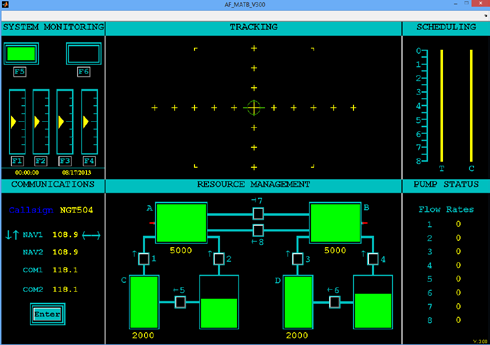
\includegraphics[width=\linewidth]{figures/matb.png}
    \caption{Main view of the MATB simulation software. }
    \label{fig:matb}
\end{figure}

The resource management subtask involves maintaining the amount of fluid that is present in two main tanks within acceptable levels. Secondary tanks are present and can be used to temporarily store fluid. The participant must toggle pumps to control the flow of fuel between the tanks. Throughout the trial, pumps will temporarily break or silently shut-off, preventing the flow of fuel through the pump. The number of these occurrences depends on the difficulty condition.

The systems monitoring subtasks is centered around two buttons and four gauges. One button must be kept on while the other button must be kept off. Throughout the simulation, the buttons change states and must be clicked, or a corresponding key pressed, to revert to the correct state. The gauges have sliders that will vary throughout the simulation. Occasionally, depending on the difficulty condition, a slider will move outside the acceptable range for the gauge and must be clicked, or the corresponding key pressed, to reset the gauge. If an out-of-state system is not addressed in a reasonable time, it is automatically reset.

The communication subtask requires the use of sound. For the duration of the simulation, the user is assigned a particular callsign for which they must listen. The communication window includes four different communication channels, each set to a particular frequency. Throughout the simulation, a recorded audio track will play, addressing a particular callsign to change a channel to a certain frequency. If the callsign matches that of the user, they must change the specified communication channel to the appropriate frequency using either the mouse or the arrow keys. If the callsign does not match that of the user, the request should be ignored. The number of true- and false-alarm requests depends on the difficulty condition. 

The tracking subtask is the only task that involves the joystick. In this subtask, the user simulates steering a plane by keeping a reticle within the acceptable parameters of the window. The amount of drifting affecting the reticle and the amount of control the joystick emits onto the reticle varies throughout the simulation in accordance to the difficulty condition.

The baseline condition for MATB involves the participant watching the screen while the simulation runs with the low condition parameters and automation enabled. This allows for the visual stimulation that would be present in performing the actions without the cognitive workload. Presented in Table~\ref{tab:matb} are the parameter values entered into the script generator of MATB to produce the trials for each load condition.

\begin{table}[h]
\centering
 \begin{adjustbox}{max width=\textwidth}
\begin{tabular}{lccccccc}
\multicolumn{1}{c}{}                                                 & \multicolumn{1}{l|}{}                                          & \multicolumn{2}{c|}{\cellcolor[HTML]{FFFFFF}\textbf{Communication}}                & \multicolumn{2}{c|}{\cellcolor[HTML]{FFFFFF}\textbf{System}}                   & \multicolumn{2}{c}{\cellcolor[HTML]{FFFFFF}\textbf{Resources}}     \\
\rowcolor[HTML]{FFFFFF} 
\multicolumn{1}{c|}{\cellcolor[HTML]{FFFFFF}\textbf{Load Condition}} & \multicolumn{1}{c|}{\cellcolor[HTML]{FFFFFF}\textbf{Tracking}} & \textbf{Target} & \multicolumn{1}{c|}{\cellcolor[HTML]{FFFFFF}\textbf{Distractor}} & \textbf{Lights} & \multicolumn{1}{c|}{\cellcolor[HTML]{FFFFFF}\textbf{Gauges}} & \textbf{Failures} & \textbf{Shut-offs}                              \\ \hline
\rowcolor[HTML]{FFFFFF} 
\multicolumn{1}{l|}{\cellcolor[HTML]{FFFFFF}\textbf{Low}}            & Low                                                            & 9               & 3                                                                & 72              & 63                                                           & 6                 & \multicolumn{1}{c|}{\cellcolor[HTML]{FFFFFF}3}  \\
\rowcolor[HTML]{EFEFEF} 
\multicolumn{1}{l|}{\cellcolor[HTML]{EFEFEF}\textbf{Medium}}         & Medium                                                         & 27              & 15                                                               & 144             & 153                                                          & 30                & \multicolumn{1}{c|}{\cellcolor[HTML]{EFEFEF}15} \\
\rowcolor[HTML]{FFFFFF} 
\multicolumn{1}{l|}{\cellcolor[HTML]{FFFFFF}\textbf{High}}           & High                                                           & 45              & 18                                                               & 216             & 243                                                          & 60                & \multicolumn{1}{c|}{\cellcolor[HTML]{FFFFFF}30} \\ \cline{2-8} 
\end{tabular}
\end{adjustbox}
\caption{Parameter values for MATB task for each load condition trial.}
\label{tab:matb}

\end{table}

\subsection{RanTask ( Auditory Task )}
The second loading task for this study is a custom tone counting task, referred to herein as RanTask. This task is an extension of the mental workload loading task used in the work of Rantanen et al.~\cite{Rantanen}. The participant is presented with three different tones in random order. The task of the participant is to count the tones that are presented and press the key corresponding to the tone when the desired count is reached.  The intended count differs with the difficulty condition. The tones correspond to the notes B at 493 Hz, F at 698 Hz, and A at 880 Hz. Each tone is presented for 1 second with a 1 second interval between tones, giving the participant 2 seconds to respond to a given tone. Each time a tone is presented, a log entry is created, recording the tone presented, its number in the sequence, and the key pressed by the participant. If a key is pressed at an incorrect time, a false-positive is logged and the sequence count for the corresponding tone is reset to prevent cascading failure, e.g. counting every 5 correctly but being off by 1 from the ground truth sequence would result in all false-positives. In the baseline trial, the participant is not required to count any of the tones, only listen. Presented in Table~\ref{tab:ran} are the desired counts for each tone in each load condition.

\begin{table}[h]
\centering
\begin{tabular}{l|ccc}
                                                                     & \multicolumn{3}{c}{\textbf{Tone Frequency}}                                     \\
\rowcolor[HTML]{FFFFFF} 
\multicolumn{1}{c|}{\cellcolor[HTML]{FFFFFF}\textbf{Load Condition}} & \textbf{Low} & \textbf{Medium} & \textbf{High}                                   \\ \hline
\rowcolor[HTML]{FFFFFF} 
\textbf{Low}                                                         & 0          & 3               & \multicolumn{1}{c|}{\cellcolor[HTML]{FFFFFF}0}  \\
\rowcolor[HTML]{EFEFEF} 
\textbf{Medium}                                                      & 0       & 7              & \multicolumn{1}{c|}{\cellcolor[HTML]{EFEFEF}0} \\
\rowcolor[HTML]{FFFFFF} 
\textbf{High}                                                        & 2         & 0              & \multicolumn{1}{c|}{\cellcolor[HTML]{FFFFFF}3} \\ \cline{2-4} 
\end{tabular}
  \caption{Desired counts of each tone for each load condition trial.}
  \label{tab:ran}
\end{table}

\subsection{NASA TLX Evaluation}
The NASA Task Load Index (TLX) survey is a means of determining the workload for a given task based on participant responses~\cite{NASA}. The procedure allows for exploring the different aspects of a task and where the underlying cognitive workload comes from. The resulting workload rating will be used to compare the difficulties of the various tasks as determined by the participants similar to the procedure used in existing studies~\cite{Ke}. The current TLX procedure consists of six subscales: Mental Demands, Physical Demands, Temporal Demands, Own Performance, Effort, and Frustration. The mental subscale measures how much mental activity was required and its complexity. Physical demands measures how much physical activity was required and how laborious it was. Temporal demands measure how much time pressure was present in the task. In the performance subscale, the participant remarks on how successful they felt they were and how satisfied they are with their performance. The effort subscale measures how hard the participant had to work to accomplish the task. The final subscale, frustration level, measures how stressed or relaxed the participant felt during the task.

\subsection{Overall Structure}
The study will take place over 4 days for each participant. Each day will require roughly 2 hours of time from the participant. The first day will consist of an introduction to the system: what sensors will be used, the intent of the study, what is expected of the participant. Training will also be conducted during the first day to familiarize the participant with the tasks to be performed. Ideally, stable performance on both tasks will be achieved as a result of training. Other studies~\cite{Wilson} have included lengthier training periods, however due to time constraints, the time required is not feasible. As such, performance results of participants will be examined and reported such as to be factored in to the discussion of overall effectiveness. The second day will begin the data collection portion of the study. Participants will be attached to the sensors and a 5 minute baseline recording using MATB will be taken. Following the baseline, the MATB task will be completed on the low-load condition for 15 minutes. After the administering of the NASA TLX and a 10 minute break, the 15 minute, low-load MATB task will be repeated. This will be followed by another NASA TLX and 10 minute break. After the break, a 5 minute baseline using RanTask will be taken. Next the participant will complete two 15 minute trials of RanTask on the low-load condition, each followed by a NASA TLX survey and separated by a 10 minute break. This marks the completion of the second day. The next two days follow the same format as Day 2 but completing medium- and high-load tasks respectively. Only a single subject will participate in the study at a time due to restrictions in the number of available sensors. The order in which the load conditions are completed follows that of an previous study~\cite{Wilson}.

%% Add a table for the schedule %%

\section{Evaluation}
Due to the multi-faceted nature of the model, evaluation will be performed on individual components as well as the system as a whole. That is, each configuration defined in the previous Classifiers section will be evaluated independently to determine effectiveness. For each evaluation, the target of a particular data point will be the difficulty condition of the trial from which the point was collected; i.e. low, medium, high. The accuracy, recall, precision, and harmonic mean metrics will be calculated by comparing the predicted level of cognitive workload with the target. As a baseline metric, the SP-ST configuration will be evaluated and compared to existing classification results such as those in the studies by Zhang et al.~\cite{Zhang} and Wilson et al.~\cite{Wilson}. Ideally the results of SP-ST will be comparable to the levels seen in previous studies, showing adequate methodology and features. The AP-CT configuration will be compared to the results found in a study by Ke et al.~\cite{Ke}, as it covers a similar area of generalizability. Meanwhile AP-ST will be compared to the results of another study~\cite{Wang_Z}. The rest of the configurations cover experimental setups that have not previously been explored. The results of these configurations will be compared to existing studies, but the comparisons may be less meaningful. A configuration is considered meaningful if the results are better than chance. Due to the 3-class nature of the study, a random assignment will have an average accuracy of 33 percent. While an accuracy higher than 33 percent is considered meaningful as it suggests a pattern has been found, accuracies closer to those found in current studies are desired.

\section{Deliverables}
Upon completion of all proposed work, a thesis report will be submitted. The thesis report will contain all background research, experiment methodology, experiment results, and discussion. Additionally, any models created and an anonymized copy of the collected data will be made available. 

\section{Timeline}
The following proposed schedule lists the major milestones of this thesis. The work is broken up into three phases: Data Collection, Model Creation, and Analysis. The writing of the thesis and required documents will be done in parallel to the main phases.

\begin{center}
\begin{tabularx}{\textwidth}{X|X}
    Date & Task\\
    \hline
    June 6 2015 & Complete thesis proposal submission, begin data collection study\\
    June 30, 2015 & Complete collection of data, begin model creation\\
    July 15, 2015 & Complete creation of models / classifiers, begin data analysis\\
    July 31, 2015 & Complete analysis of model results, begin thesis wrap-up\\
    August 10, 2015 & Defend thesis\\
\end{tabularx}
\end{center}


\bibliography{references}

\end{document}




















